% ReportKit example: equity-research publication type + institutional-research
% theme. Step 5 of
% docs/superpowers/specs/2026-09-09-reportkit-institutional-theme-and-equity-profile-spec.md
% ("Fixtures + QA + skill guidance"). Fictional content (Nexa Cloud
% Solutions / NXCL), inspired by the spec's Appendix A prototype but
% rebuilt from only the public primitives Steps 1-4 shipped
% (researchfrontpage/researchheadline/ratingstrip/whatschanged/exhibit/
% exhibitpair/exhibitgrid/financialtable/financialmodelpage/bullcase-
% basecase-bearcase, apply_theme()/risk_reward_chart() in figures.py) --
% no page-specific coordinates, local font patches, bespoke chart styling,
% or raw minipage layouts, per spec section 28's Definition of Done.
%
% -----------------------------------------------------------------------------
% Fixture arithmetic reconciliation (open question 6)
% -----------------------------------------------------------------------------
% Appendix A's own numbers are internally inconsistent across three islands
% (front page/Exhibit 4's FY27E EBITDA 691 / EPS 2.95; Exhibit 5's model,
% self-consistent on FY27E EBITDA 917 / EPS 2.27; Exhibit 6's valuation,
% which needs 122 diluted shares to reach $245 against the model's 241, and
% whose Value/Share column sums to $233, not $245). This fixture picks
% Exhibit 5's income statement as the single anchor -- it is the most
% granular island (quarterly figures sum to the annual ones it reports) --
% and derives every other number in the document from it:
%
%   - Front page / sidebar / Exhibit 4's "New" columns use the model's own
%     FY25A-FY28E Revenue/Subscription/AI Orchestration/Services/Adjusted
%     EBITDA/EPS exactly. (Exhibit 4's revenue-line New figures already
%     matched the model in Appendix A; only its EBITDA/EPS rows and the
%     front page/sidebar needed correcting from 691/2.95 to 917/2.27.)
%   - Exhibit 4/front-page "Old" (prior-estimate) figures are independent,
%     plausible prior numbers -- there is no earlier fixture they need to
%     reconcile against -- chosen so New vs Old tells the same "estimates
%     trimmed, mix improves" story Appendix A's prose already tells.
%     FY26E EPS Old ($1.43) is bottom-up from the sidebar's own prior
%     quarterly EPS estimates (0.26 actual + 0.34 + 0.38 + 0.45), not a
%     separate guess.
%   - Exhibit 2 (platform mix) percentages are each year's
%     Subscription/AI Orchestration/Services revenue over total revenue,
%     computed from the model, not eyeballed.
%   - Exhibit 6 (renumbered Exhibit 7 here, since this fixture has an
%     extra usage-index exhibit Appendix A's page 2 also had) is rebuilt
%     as three EV/Sales lines (all using the model's actual FY27E segment
%     revenue, not a fourth, unreconciled "Services EBITDA" plug) at
%     21.4x/30.0x/5.0x, chosen so Enterprise Value ($57,141M) + Net Cash
%     ($1,860M) = Equity Value ($59,001M), divided by the model's own
%     241M FY27E diluted shares = $244.90/share -- rounded to the $245
%     published target used consistently everywhere else in the document
%     (front page, rating strip, whatschanged, risk/reward chart). The
%     Value/Share column is extended with an explicit Net Cash per share
%     row (Appendix A left this implicit, which is exactly how its own
%     $233-vs-$245 gap went unnoticed) so the column's own numbers are
%     auditable: they sum to $244.82 (2dp rounding noise against the
%     unrounded $244.90), not silently off by 5% the way Appendix A's did.
%   - The risk/reward page's Bull/Base/Bear narrative multiples are
%     restated as EV/Sales on FY28E consolidated revenue ($3,165M) rather
%     than Appendix A's EV/EBITDA framing (whose Base case reused the
%     model's FY27E EBITDA number under a "CY28E" label) -- consistent
%     with Exhibit 7's own methodology and exactly reproducing each
%     scenario's price target from the same shares/net-cash basis:
%     Bear $135 -> 9.7x, Base $245 -> 18.1x, Bull $310 -> 23.0x.
%
% See figures.py for the figure-level arithmetic (platform mix, gross
% margin) built the same way.
\documentclass[theme=institutional-research,publication-type=equity-research]{reportkit}

\setreportkitleftheader{Nexa Cloud Solutions, Inc. (NXCL)}
\setreportkitfooter{ReportKit Research -- Fictional demonstration publication}
\setreportkitversion{v1.0}
\setreportkitsubject{Equity research update}
\setreportkitkeywords{ReportKit, equity research, institutional-research theme}
\setreportkitfontpolicy{fallback}

\title{AI Infrastructure Demand Is Holding Up Better Than Feared; Services Mix Provides an Offset}
\author{ReportKit Research}
\date{8 September 2026}

\begin{document}

\begin{researchfrontpage}
\researchkicker{Enterprise Software / North America}
\researchheadline{AI Infrastructure Demand Is Holding Up Better Than Feared; Services Mix Provides an Offset}
\researchdeck{We trim FY27 infrastructure growth assumptions after channel checks point to slower enterprise deployments, but raise our services estimates as AI orchestration usage remains resilient. Lower hardware-linked contribution is more than offset by recurring platform revenue, keeping our price target at \$245.}

\begin{ratingstrip}[itemcount=4]
\ratingitem{Stock Rating}{\color{Accent}Overweight}
\ratingitem{Price Target}{\$245}
\ratingitem{Reference Price}{\$182.50}
\ratingitem{Implied Upside}{34.3\%}
\end{ratingstrip}

\begin{whatschanged}
\change{FY27 Revenue (\$M)}{2,610}{2,540}
\change{FY27 EPS (\$)}{\$2.35}{\$2.27}
\change{Price Target}{\$245}{\$245}
\end{whatschanged}

\begin{researchmain}
\textbf{Enterprise AI demand is slowing, not breaking.} Our channel work indicates large customers are extending deployment timelines by one to two quarters, but the underlying pipeline remains intact. Usage-based orchestration revenue continues to grow faster than subscription seats, suggesting customers are consolidating workloads rather than abandoning AI projects -- see Exhibit 1.

\textbf{Services and platform mix now matter more than unit growth.} We forecast AI Orchestration and Token Routing to rise to 28\% of revenue by FY27E from 21\% in FY25A (Exhibit 2), a mix shift that supports gross margin expansion (Exhibit 3) even alongside a more conservative infrastructure outlook.

\textbf{We see limited downside to estimates from current checks.} Our FY27E revenue estimate falls 2.7\%, but Adjusted EBITDA declines only about 1\% as lower-margin, hardware-linked activity accounts for most of the revision (Exhibit 4).

\textbf{The key debate is duration, not direction.} Investors appear to be discounting a full normalization in enterprise AI spending. Our work suggests the more likely path is a slower but longer adoption cycle, with services, security, and inference routing becoming the primary value drivers over the next 24 months.
\end{researchmain}\begin{researchsidebar}
\begin{analystblock}
\sidebarlabel{ReportKit Research LLC}\\
\sidebarvalue{Alexander Vance, CFA}\\
\textcolor{Muted}{Equity Analyst}\\
alexander.vance@example.com\\[5pt]
\sidebarvalue{Sarah Jenkins}\\
\textcolor{Muted}{Research Associate}\\
sarah.jenkins@example.com
\end{analystblock}

\begin{marketdatablock}
\sidebarvalue{Nexa Cloud Solutions (NXCL)}\\[2pt]
\sidebarrow{Stock Rating}{Overweight}
\sidebarrow{Industry View}{Attractive}
\sidebarrow{Price Target}{\$245.00}
\sidebarrow{Share Price}{\$182.50}
\sidebarrow{Market Cap (\$M)}{42,850}
\sidebarrow{52-Week Range}{\$124.10--\$195.40}
\end{marketdatablock}

\begin{estimatesblock}
\noindent{\sidebarvalue{Fiscal Year Ending}}\\[2pt]
\begin{tabularx}{\linewidth}{@{}Yrrrr@{}}
& \textbf{2025A} & \textbf{2026E} & \textbf{2027E} & \textbf{2028E}\\
\midrule
EPS (\$) & 0.57 & 1.39 & 2.27 & 3.18\\
P/E (x) & 320 & 131 & 80 & 57\\
Revenue (\$M) & 1,520 & 1,985 & 2,540 & 3,165\\
Adj. EBITDA (\$M) & 366 & 636 & 917 & 1,217\\
\end{tabularx}
\end{estimatesblock}

\begin{estimatesblock}
\noindent{\sidebarvalue{FY26 Quarterly EPS (\$)}}\\[2pt]
\begin{tabularx}{\linewidth}{@{}Yrrr@{}}
& \textbf{2Q26E} & \textbf{3Q26E} & \textbf{4Q26E}\\
\midrule
Prior & 0.34 & 0.38 & 0.45\\
Current & 0.32 & 0.37 & 0.44\\
\end{tabularx}
\vspace{2pt}
\sidebarlabel{1Q26A actual \$0.26, unchanged.}
\end{estimatesblock}

\vfill
{\rkdisclosuresize\color{Muted}ReportKit Research does and seeks to do business with companies covered in its research. Investors should consider this report as only a single factor in making an investment decision. This is a fictional demonstration publication; see the disclosures on the final page.\par}
\end{researchsidebar}
\end{researchfrontpage}

\newpage
\section{Analysis}

\begin{fullwidthexhibit}
\begin{exhibit}[
  title={Enterprise AI usage remains resilient even as deployment cycles lengthen},
  source={Company data; ReportKit Research estimates.},
  label={fig:usage-index}
]
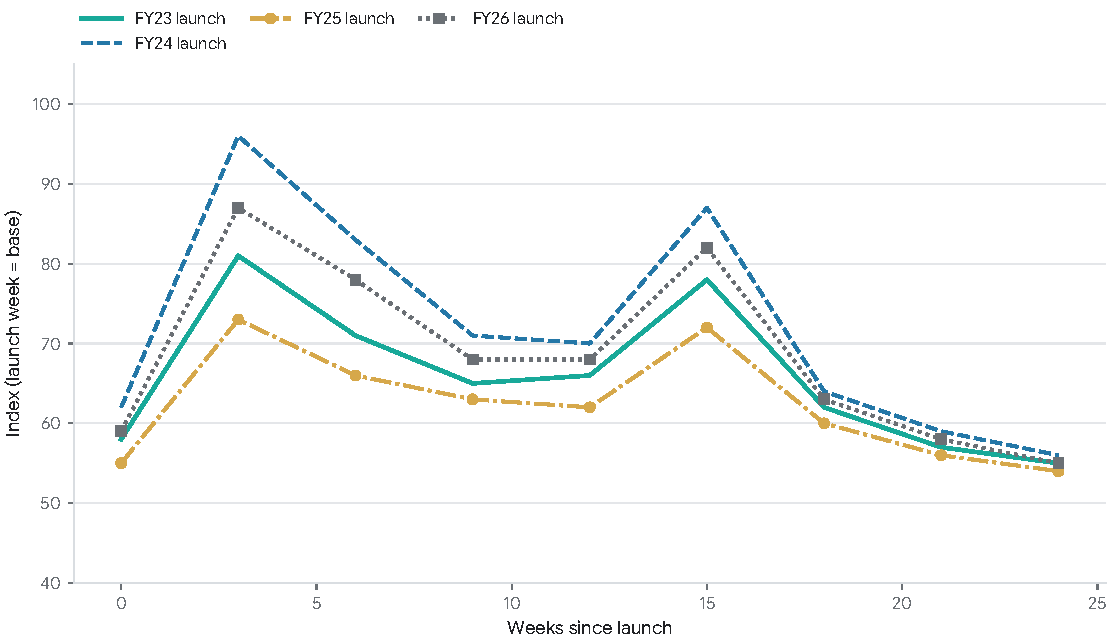
\includegraphics[width=\linewidth]{figures/usage_index.pdf}
\end{exhibit}
\end{fullwidthexhibit}

\begin{exhibitpair}
\exhibitpane{
\begin{exhibit}[
  title={Platform mix is rising as a share of total revenue},
  source={Company data; ReportKit Research estimates.},
  label={fig:platform-mix}
]
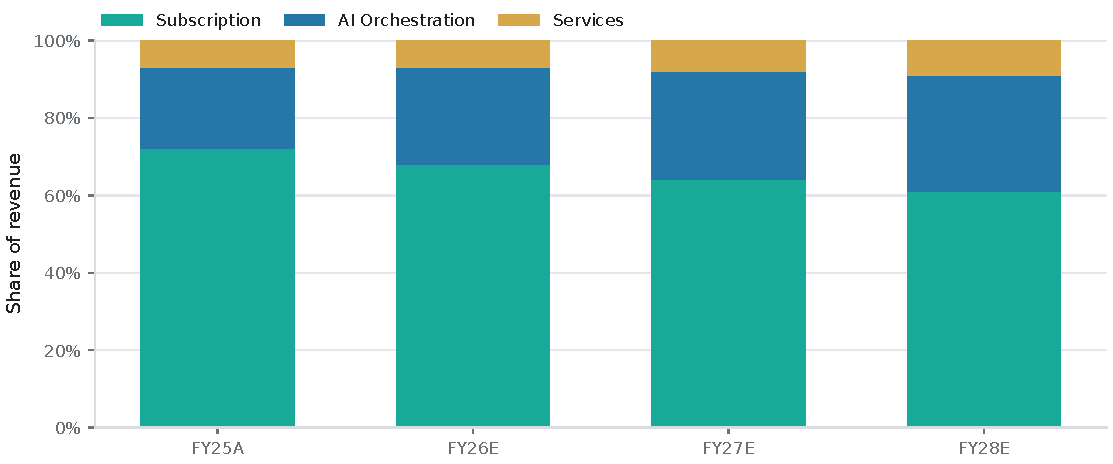
\includegraphics[width=\linewidth]{figures/platform_mix.pdf}
\end{exhibit}
}
\exhibitpane{
\begin{exhibit}[
  title={Gross margin expands despite slower infrastructure growth},
  source={Company data; ReportKit Research estimates.},
  label={fig:gross-margin}
]
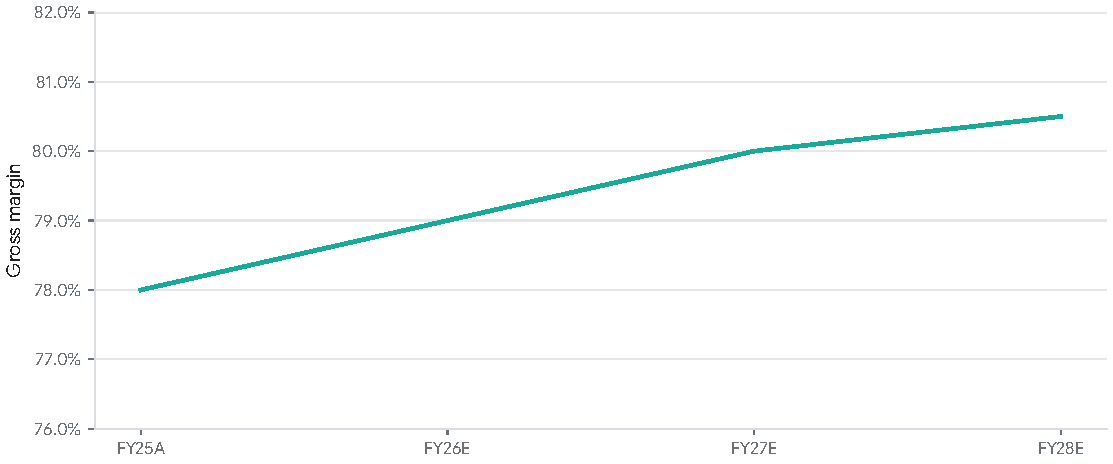
\includegraphics[width=\linewidth]{figures/gross_margin.pdf}
\end{exhibit}
}
\end{exhibitpair}

\begin{fullwidthexhibit}
\begin{exhibit}[
  title={Estimate revisions are concentrated in lower-margin services activity},
  source={ReportKit Research estimates.},
  label={tab:estimate-revisions}
]
\begin{financialtable}
\begin{tabularx}{\linewidth}{@{}Yrrrrrrrrr@{}}
\toprule
 & \multicolumn{3}{c}{\textbf{FY26E}} & \multicolumn{3}{c}{\textbf{FY27E}} & \multicolumn{3}{c}{\textbf{FY28E}}\\
\cmidrule(lr){2-4}\cmidrule(lr){5-7}\cmidrule(lr){8-10}
\textbf{Metric} & New & Old & \% Chg & New & Old & \% Chg & New & Old & \% Chg\\
\midrule
Revenue (\$M) & 1,985 & 2,010 & -1.2\% & 2,540 & 2,610 & -2.7\% & 3,165 & 3,250 & -2.6\%\\
Subscription & 1,350 & 1,360 & -0.7\% & 1,626 & 1,650 & -1.5\% & 1,940 & 1,970 & -1.5\%\\
AI Orchestration & 496 & 490 & +1.2\% & 711 & 690 & +3.0\% & 950 & 920 & +3.3\%\\
Services & 139 & 160 & -13.1\% & 203 & 270 & -24.8\% & 275 & 360 & -23.6\%\\
Adjusted EBITDA (\$M) & 636 & 631 & +0.8\% & 917 & 926 & -1.0\% & 1,217 & 1,233 & -1.3\%\\
EPS (\$) & 1.39 & 1.43 & -2.8\% & 2.27 & 2.35 & -3.4\% & 3.18 & 3.28 & -3.0\%\\
\bottomrule
\end{tabularx}
\end{financialtable}
\end{exhibit}
\end{fullwidthexhibit}

\newpage
\section{NXCL Risk/Reward}

\begin{researchmain}
\begin{fullwidthexhibit}
\begin{exhibit}[
  title={Services mix is underappreciated by investors},
  source={Company filings; ReportKit Research estimates.},
  label={fig:risk-reward}
]
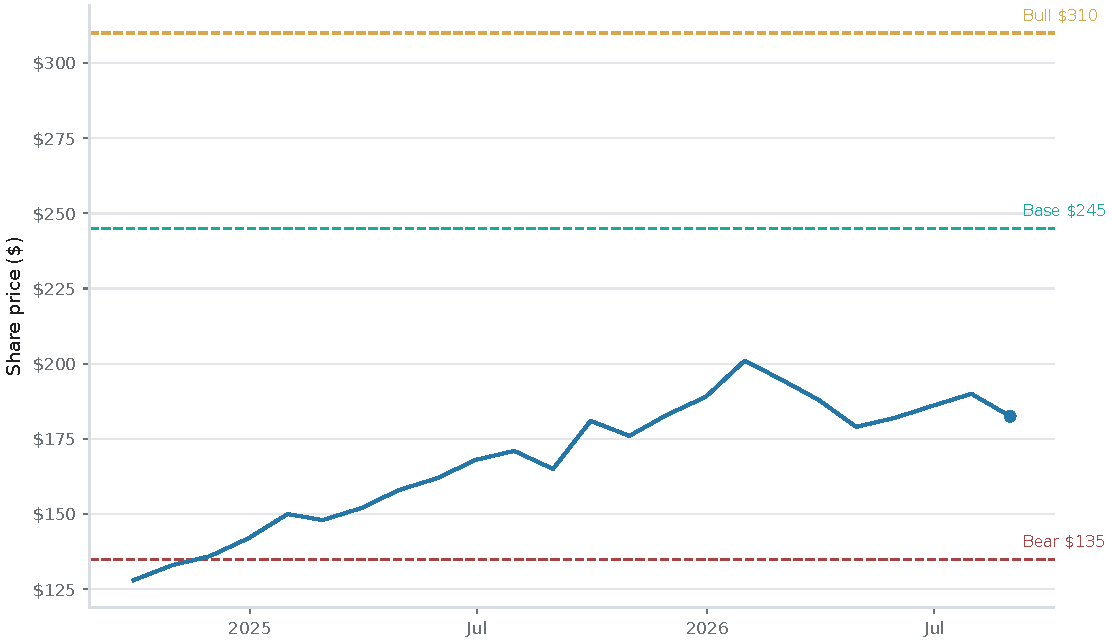
\includegraphics[width=\linewidth]{figures/risk_reward.pdf}
\end{exhibit}
\end{fullwidthexhibit}

\rksubheading{Price Target}
Derived from the base-case scenario in our sum-of-the-parts framework (Exhibit 7). At \$245, our target implies roughly 34\% upside from the current \$182.50 share price.

\bullcase{\$310}{23.0x FY28E EV/Sales on \$3.2B revenue. Platform adoption accelerates, AI orchestration becomes the primary workload-control layer for large enterprises, and net retention stabilizes above 135\%. Gross margin exceeds 81\% as usage scales with limited incremental infrastructure cost.}
\basecase{\$245}{18.1x FY28E EV/Sales on \$3.2B revenue. Enterprise deployments remain slower than the 2024--25 pace, but recurring platform revenue and usage-based routing support high-teens growth with steady margin expansion.}
\bearcase{\$135}{9.7x FY28E EV/Sales on \$3.2B revenue. A broader IT budget slowdown delays production deployments, hyperscalers bundle competing routing software, and customers consolidate vendors. Revenue growth falls to the low teens and margin expansion stalls.}
\end{researchmain}\begin{researchsidebar}
\sffamily\rksidebarsize\color{Ink}
\rksubheading{Investment Thesis}
\begin{itemize}
\item Nexa occupies a valuable control point between enterprise applications and multiple model providers.
\item Services mix should increase revenue visibility and reduce quarterly deployment cyclicality.
\item Improving gross margin and sales efficiency support durable free-cash-flow conversion.
\end{itemize}

\rksubheading{Key Debates}
\textbf{Can AI infrastructure spending reaccelerate?} Yes, but we expect the recovery to be driven by production workloads rather than experimentation.\par\vspace{4pt}
\textbf{Can hyperscalers commoditize routing?} Partly -- we think multi-cloud governance and data-security requirements preserve a role for independent control-plane software.

\rksubheading{Potential Catalysts}
\begin{itemize}
\item Faster enterprise migration from pilot to production.
\item Expanded co-sell agreements with major cloud providers.
\item Capital return once free cash flow exceeds \$700M.
\end{itemize}

\rksubheading{Risks to Price Target}
\begin{itemize}
\item Hyperscaler bundling and pricing pressure.
\item Customer concentration and delayed renewals.
\item Regulatory constraints on enterprise AI deployment.
\end{itemize}

\vspace{6pt}
\rksubheading{Business Mix}
\begin{minipage}[t]{\linewidth}
  \centering
  
\includegraphics[width=1.8in]{figures/business_mix.pdf}
\end{minipage}
\sidebarrule
\begin{sidebarrow}{Consulting}{52\%}\end{sidebarrow}
\begin{sidebarrow}{Managed Services}{48\%}\end{sidebarrow}
\end{researchsidebar}

\newpage
\section{NXCL Financial Model}

\begin{fullwidthexhibit}
\begin{exhibit}[
  title={Income statement and key operating metrics},
  source={Company data; ReportKit Research estimates.},
  label={tab:financial-model}
]
\begin{financialmodelpage}
\begin{tabular}{@{}lrrrrrrrrrrrr@{}}
\toprule
\textbf{\$M except per-share data} & \textbf{1Q25A}&\textbf{2Q25A}&\textbf{3Q25A}&\textbf{4Q25A}&\textbf{1Q26A}&\textbf{2Q26E}&\textbf{3Q26E}&\textbf{4Q26E}&\textbf{2025A}&\textbf{2026E}&\textbf{2027E}&\textbf{2028E}\\
\midrule
\textbf{Revenue} & 342&366&391&421&442&478&510&555&1,520&1,985&2,540&3,165\\
Subscription & 251&265&278&300&307&326&341&376&1,094&1,350&1,626&1,940\\
AI Orchestration & 69&78&85&87&103&116&131&146&319&496&711&950\\
Services & 22&23&28&34&32&36&38&33&107&139&203&275\\
Revenue growth (\%) & 34&33&32&34&29&31&30&32&33&31&28&25\\
\midrule
Cost of revenue & 78&82&86&89&94&101&107&115&335&417&508&617\\
\textbf{Gross profit} & 264&284&305&332&348&377&403&440&1,186&1,568&2,032&2,548\\
Gross margin (\%) & 77.2&77.6&78.0&78.8&78.7&78.9&79.0&79.3&78.0&79.0&80.0&80.5\\
\midrule
R\&D & 96&99&102&113&111&116&121&128&410&476&559&665\\
Sales \& marketing & 113&118&123&132&128&133&139&145&486&545&635&728\\
G\&A & 34&35&37&41&39&40&41&43&147&163&191&228\\
\textbf{Operating income} & 21&32&43&46&70&88&102&124&143&384&647&927\\
Operating margin (\%) & 6.1&8.7&11.0&10.9&15.8&18.4&20.0&22.3&9.4&19.3&25.5&29.3\\
\midrule
D\&A & 20&22&23&24&24&25&26&27&89&102&112&121\\
Stock compensation & 31&33&35&36&36&37&38&39&135&150&158&169\\
\textbf{Adjusted EBITDA} & 72&87&101&106&130&150&166&190&366&636&917&1,217\\
EBITDA margin (\%) & 21.1&23.8&25.8&25.2&29.4&31.4&32.5&34.2&24.1&32.0&36.1&38.5\\
\midrule
Interest \& other & 5&5&6&6&7&7&8&8&22&30&36&42\\
Pretax income & 26&37&49&52&77&95&110&132&165&414&683&969\\
Taxes & 5&7&10&10&15&19&22&26&32&82&136&194\\
\textbf{Net income} & 21&30&39&42&62&76&88&106&133&332&547&775\\
Diluted shares (M) & 235&236&236&237&237&238&238&239&236&238&241&244\\
\textbf{EPS (\$)} & 0.09&0.13&0.17&0.18&0.26&0.32&0.37&0.44&0.57&1.39&2.27&3.18\\
\bottomrule
\end{tabular}
\end{financialmodelpage}
\end{exhibit}
\end{fullwidthexhibit}

\begin{fullwidthexhibit}
\begin{exhibit}[
  title={Sum-of-the-parts valuation supports a \$245 price target},
  source={Company data; ReportKit Research estimates. Figures are fictional and for design demonstration only. Component value-per-share figures sum to \$244.82 (2dp rounding against the unrounded \$244.90) before rounding to the \$245 published target.},
  label={tab:valuation}
]
\begin{financialtable}
\begin{tabularx}{\linewidth}{@{}Yrrrrr@{}}
\toprule
\textbf{Segment / Metric} & \textbf{2027E Rev.} & \textbf{Multiple} & \textbf{EV (\$M)} & \textbf{Weight} & \textbf{Value/Share}\\
\midrule
Core Subscription & 1,626 & 21.4x EV/Sales & 34,796 & 61\% & \$144.38\\
AI Orchestration & 711 & 30.0x EV/Sales & 21,330 & 37\% & \$88.51\\
Services & 203 & 5.0x EV/Sales & 1,015 & 2\% & \$4.21\\
\midrule
\textbf{Enterprise Value} & & & \textbf{57,141} & \textbf{100\%} & \\
(+) Net cash & & & 1,860 & & \$7.72\\
\midrule
\textbf{Equity Value} & & & \textbf{59,001} & & \\
Diluted shares (M) & & & 241 & & \\
\textbf{Price Target (rounded)} & & & & & \textbf{\$245}\\
\bottomrule
\end{tabularx}
\end{financialtable}
\end{exhibit}
\end{fullwidthexhibit}

\vfill
{\rkdisclosuresize\color{Muted}\textbf{ANALYST CERTIFICATION AND IMPORTANT DISCLOSURES:} The analyst(s) responsible for the preparation of this report certify that the views expressed accurately reflect their personal views about the subject company. Nexa Cloud Solutions, NXCL, ReportKit Research, and every named individual in this document are fictional. This document is a design-system demonstration fixture for the ReportKit institutional-research theme and equity-research publication type and is not investment advice.\par}

\end{document}
